\section{Обеспечение электробезопасности при эксплуатации проектируемого устройства}

Первоначальные стадии разработки дипломного проекта выполнялись на предприятии «Информационные системы Байкард» во время прохождения преддипломной практики. Для использования системы необходимо произвести настройку серверов, терминалов для доставки билетов. Таким образом, нужно иметь дело с электрооборудованием. В настоящем разделе рассматриваются вопросы, связанные с обеспечением электробезопасности на предприятии.

В качестве примера рассмотрим терминал для доставки билетов. Схема электропитания терминала изображена на рисунке ~\ref{ot-el-schema}

\begin{figure}
  	\label{ot-el-schema}
  	\centering
  	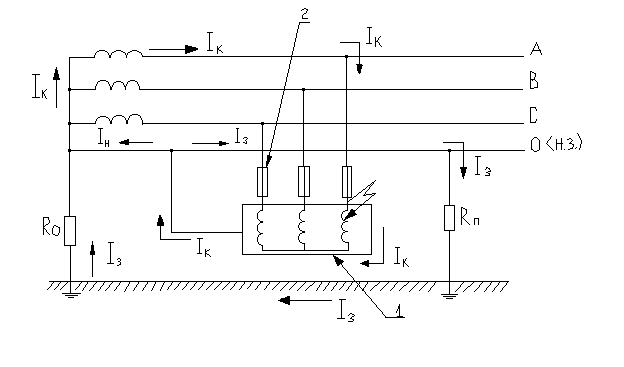
\includegraphics[width=1\textwidth]{images/ot-el-schema.png}
  	\caption{Схема электропитания}
\end{figure}

Внутренние устройства монтируются в корпус, у которого есть подключение к стандартной сети 220 В. Основные свойства блока питания YP-350J-AA:

\begin{itemize}
    \item универсальный вход 100…264 В переменного тока; 
    \item выходная мощность: 350 Вт; 
    \item не боится провалов входного напряжения; 
    \item встроенный корректор коэффициента мощности; 
    \item коэффициент мощности >0,95; 
    \item комплекс защит: от перегрузки и перенапряжения.
\end{itemize}

Поражение электрическим током возможно как при случайном прикосновении его  непосредственно к токоведущим частям, так и к неметаллическим нетоковедущим элементам электрооборудования (к корпусу электрических машин, трансформаторов, светильников и т.п.), которые могут оказаться под напряжением в результате какой – либо аварийной ситуации (замыкания фазы на корпус, повреждение изоляции и т.п.).

Оценка опасности электропоражения заключается в сравнении максимально возможных токов электропоражения, полученных с помощью измерения или расчёта, с предельно допустимыми их значениями. Предельно допустимые напряжения прикосновения \( \text{U}_{\text{пр}} \) и токи, проходящие через человека \( \text{I}_{\text{h пд}} \) при нормальном (неаварийном) режиме работы электроустановки приведены в таблице ~\ref{ot-tab}:

\begin{table}[h]
\label{ot-tab}
\center
\begin{xtabular}{|l|l|l|ll}
	\cline{1-3}
	\multirow{2}{*}{Род и частота тока} & \multicolumn{2}{l|}{Предельно допустимые значения} &  &  \\ \cline{2-3}
	& \multicolumn{1}{|>{}p{0.20\textwidth}|} {Uпр}                      & \multicolumn{1}{|>{}p{0.20\textwidth}|} {Ih}                      &  &  \\ \cline{1-3}
	\multicolumn{1}{|>{}p{0.33\textwidth}|}{Переменный, 50Гц} & 2 & 0,3 &  &  \\ \cline{1-3}
	\multicolumn{1}{|>{}p{0.33\textwidth}|}{Постоянный} & 8 & 1,0 &  &  \\ \cline{1-3}
\end{xtabular}
\end{table}

Оценка опасности позволяет определить необходимость применения способов и средств защиты, а возможные или фактические и предельно допустимые значения тока, проходящего через тело человека, и напряжения прикосновения служат исходными данными для их выбора, проектирования и расчёта.

Защитное зануление и заземление являются наиболее распространенными, весьма эффективными и простыми мерами защиты от поражения электрическим током при появлении напряжения на металлических нетоковедущих частях (металлических корпусах оборудования).

Опасность поражения электрическим током при прикосновении к корпусу и другим нетоковедущим частям электрооборудования, оказавшимся под напряжением, может быть устранена быстрым отключением поврежденного электрооборудования от питающей сети. Для этой цели используется зануление, принципиальная схема которого в сети трехфазного тока показана на рисунке 2:

\begin{figure}
  	\label{ot-zanul}
  	\centering
  	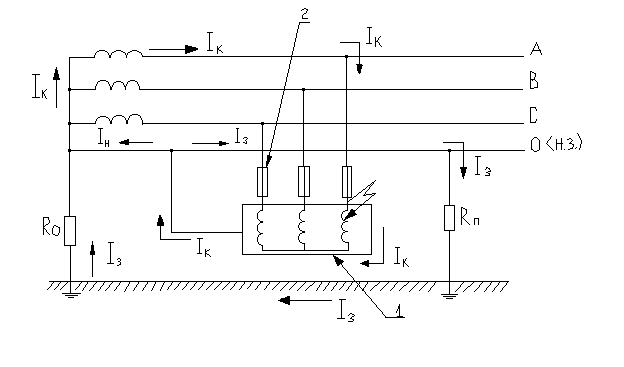
\includegraphics[width=1\textwidth]{images/ot-zanul.png}
  	\caption{Принципиальная схема зануления}
\end{figure}

Обозначения на схеме (рисунок 2):

1 --- корпус;

2 --- аппараты защиты от токов короткого замыкания (предохранители, автоматические выключатели.);

\( \text{R}_{\text{0}} \) --- сопротивление заземления нейтрали источника тока;

\( \text{R}_{\text{п}} \) --- сопротивление повторного заземления нулевого защитного проводника;

\( \text{I}_{\text{к}} \) --- ток короткого замыкания;

\( \text{I}_{\text{н}} \) --- часть тока короткого замыкания, протекающая через нулевой проводник;

\( \text{I}_{\text{з}} \) --- часть тока короткого замыкания, протекающая через землю;

0 (н.з.) --- нулевой защитный проводник.

Зануление – это преднамеренное электрическое соединение с нулевым защитным проводником металлических нетоковедущих частей, которые могут оказаться под напряжением.
Принцип действия зануления – превращение замыкания на корпус в однофазное короткое замыкание (между фазным и нулевым проводником) с целью вызвать большой ток, способный обеспечить срабатывание защиты и автоматически отключить поврежденное электрооборудование от питающей сети. В качестве отключающих аппаратов используются: плавкие предохранители, автоматические выключатели, магнитные пускатели и т.д. При этом необходимо учесть, что с момента возникновения аварии (замыкания на корпус) и до момента автоматического отключения поврежденного оборудования от сети имеется небольшой промежуток времени, в течение которого прикосновение к корпусу опасно, так как корпус находится под напряжением Uф  (рисунок 2)  и отключение его от сети еще не произошло. В этот период сказывается защитная функция заземления корпуса оборудования через нулевой защитный проводник.

Принцип действия зануления – превращение замыкания на корпус в однофазное короткое замыкание (между фазным и нулевым проводником) с целью вызвать большой ток, способный обеспечить срабатывание защиты и автоматически отключить поврежденное электрооборудование от питающей сети. В качестве отключающих аппаратов используются: плавкие предохранители, автоматические выключатели, магнитные пускатели и т.д. При этом необходимо учесть, что с момента возникновения аварии (замыкания на корпус) и до момента автоматического отключения поврежденного оборудования от сети имеется небольшой промежуток времени, в течение которого прикосновение к корпусу опасно, так как корпус находится под напряжением Uф  (рисунок 2)  и отключение его от сети еще не произошло. В этот период сказывается защитная функция заземления корпуса оборудования через нулевой защитный проводник.

Отключение поврежденной установки от питающей сети произойдет, если значение тока однофазного короткого замыкания, которое искусственно создается в цепи, будет больше (или равно) значения тока срабатывания автоматического выключателя (или номинального тока плавкой вставки предохранителя) и выполняется следующее условие:

где k --- коэффициент кратности тока, выбирается в зависимости от типа защиты электроустановки.

Для расчета зануления используем рисунок 3.

\begin{figure}
  	\label{ot-zanul}
  	\centering
  	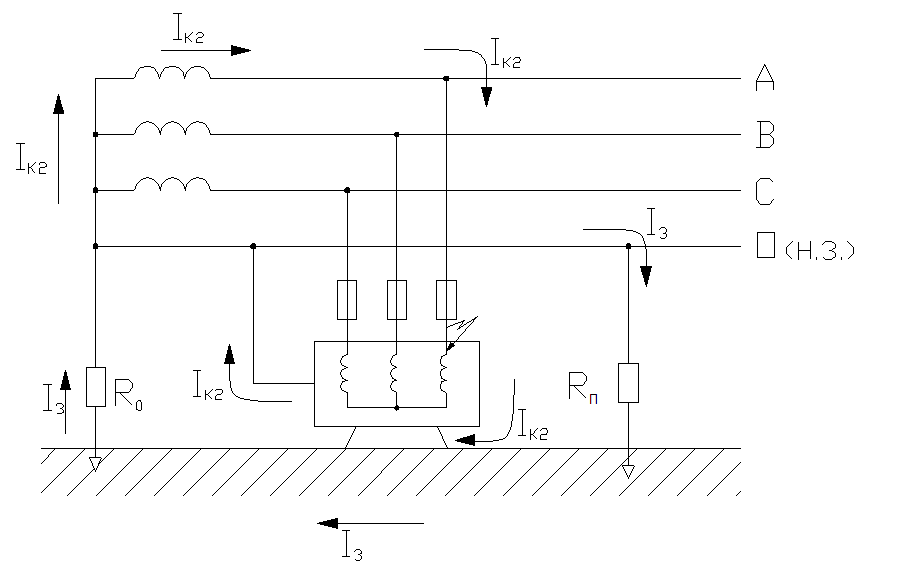
\includegraphics[width=1\textwidth]{images/ot-zanul2.png}
  	\caption{Зануление}
\end{figure}

Расчет зануления сводится к проверке соблюдения следующего условия:

\begin{displaymath}
  \text{I}_{\text{К2}} >= \text{I}_{\text{К1}}
\end{displaymath}

Для этого необходимо определить:

\begin{enumerate}
	\item наименьшее допустимое значение тока (\(\text{I}_{\text{К1}}\)) короткого замыкания, при котором произойдет срабатывание защиты и поврежденное оборудование отключится от сети;
	\item действительное значение тока однофазного короткого замыкания, которое будет иметь место в схеме при возникновении аварии (\(\text{I}_{\text{К2}}\)).
\end{enumerate}

Определяем величину тока:

\begin{displaymath}
  \text{I}_{\text{К1}} = k\cdot\text{I}_\text{ном},
\end{displaymath}

где \(\text{I}_\text{ном}\) --- номинальный ток плавкой вставки предохранителя электродвигателя, \(\text{I}_\text{ном}\) = 10А;

k --- коэффициент кратности, k = 1,25.

\begin{displaymath}
  \text{I}_{\text{К1}} = 1,25\cdot10 = 12,5\text{ (А)}
\end{displaymath}

Определяем полное сопротивление петли “фаза–нуль”:

\begin{displaymath}
  \text{Z}_\text{П} = \sqrt{(\text{R}_\text{ф}+\text{R}_\text{нз})^2+(\text{Х}_\text{ф}+\text{Х}_\text{нз}+\text{Х}_\text{п})^2},
\end{displaymath}

где \(\text{Р}_\text{ф}\), \(\text{Р}_\text{нз}\) --- активные сопротивления фазного и нулевого защитного проводников, \(\text{Р}_\text{ф}\) = 0,09 Ом, \(\text{Р}_\text{нз}\) = 0,308 Ом;

\(\text{Х}_\text{ф}\), \(\text{Х}_\text{нз}\) --- внутренние индуктивные сопротивления фазного и нулевого защитного проводников, \(\text{Х}_\text{ф}\) = 0,033 Ом, \(\text{Х}_\text{нз}\) = 0,308 Ом;

\(\text{Х}_\text{п}\) --- внешнее индуктивное сопротивление петли “фаза–нуль” (0,02 Ом).

\begin{displaymath}
  \text{Z}_\text{П} = \sqrt{(0,9+0,308)^2+(0,033+0,308+0,02)^2} = 1,21 \text{ (Ом)}.
\end{displaymath}

Находим действительное значение тока однофазного короткого замыкания, проходящего в схеме в аварийном режиме:

\begin{displaymath}
  \text{I}_\text{К2} = \frac{\text{U}_\text{Ф}}{\frac{\text{Z}_\text{T}}{3}+\text{Z}_\text{П}}
\end{displaymath}

где \(\text{U}_\text{ф}\) --- фазное напряжение, \(\text{U}_\text{ф}\) = 220 В;

\(\text{Z}_\text{П}\) --- полное сопротивление петли “фаза–нуль”;

\(\text{Z}_\text{T}\) --- полное сопротивление трансформатора, \(\text{Z}_\text{T}\) = 1,237 Ом.

\begin{displaymath}
  \text{I}_\text{К2} = \frac{220}{\frac{1,237}{3}+1,21} = 136 \text{ (А)}
\end{displaymath}

Так как условие \(\text{I}_\text{К2}\) >= \(\text{I}_\text{К1}\) выполняется, следовательно, отключающая способность зануления обеспечена, и защитный проводник выбран правильно.


